% !TEX root = BA-Bauer.tex

\subsection{LED}

Licht emittierende Dioden (LED) sind ein essentieller Bestandteil der Benutzerschnittstelle für die Lokalisierung von Fehlern und dienen der Überwachung der laufenden Aufnahme oder Wiedergabe aus kleiner und großer Distanz. Insgesamt werden fünf LEDs in vier verschiedenen Farben (blau, orange, grün und rot) verbaut, um dem Benutzer eine Unterscheidung auch auf große Distanz zum Gerät möglichst einfach zu machen. Ziel ist es, eine möglichst hardwarenahe Rückmeldung an den Benutzer zu geben. Tabelle \ref{table:LED} fasst die Funktionen der einzelnen LEDs zusammen. 
\begin{table}[h]
	\begin{center}
		\caption{LED Funktionen}
		\begin{tabular}{l | l}
				\textbf{LED-Farbe} & \textbf{Funktion}\\
				\hline
				blau & Eingeschaltet bei aktiver Spannungsversorgung des Geräts\\
				rot & Zustandsänderung bei eingehendem DMX-Datenpaket\\
				blau & Zustandsänderung bei ausgehendem DMX-Datenpaket\\
				orange & Eingeschaltet bei Schreib- oder Lesevorgängen der SD-Karte\\
				grün & Allgemeine Zustandsanzeige
		\end{tabular}
		\label{table:LED}
	\end{center}
\end{table}
Die erste blaue LED wird direkt an die 5\,V Versorgungsspannung, ausgehend von der USB-Buchse über einen Widerstand zur Strombegrenzung, angeschlossen. Dadurch kann sehr einfach festgestellt werden, ob das Gerät mit Spannung versorgt wird, unabhängig von der Funktion der restlichen Schaltung. Die zweite blaue und die rote LED müssen zwangsläufig per Software geschaltet werden, da der XLR-Ein- und Ausgang parallel verbunden sind. Eine Unterscheidung von ein- bzw. ausgehenden Daten ist so nicht möglich. Zudem haben Tests gezeigt, dass das direkte Verbinden einer LED mit einer Datenleitung die LED nicht intensiv genug zum leuchten bringt. Gleiches gilt für die orange LED. In einer Weiterentwicklung des Gerätes kann z.B. mithilfe einer monostabilen Kippstufe, wie einem NE555 IC \cite{NE555}, welche den eingeschalteten Zustand einer LED verlängern kann, eine hardwarenähere Lösung realisiert werden.
\begin{figure}[h]
	\begin{center}
		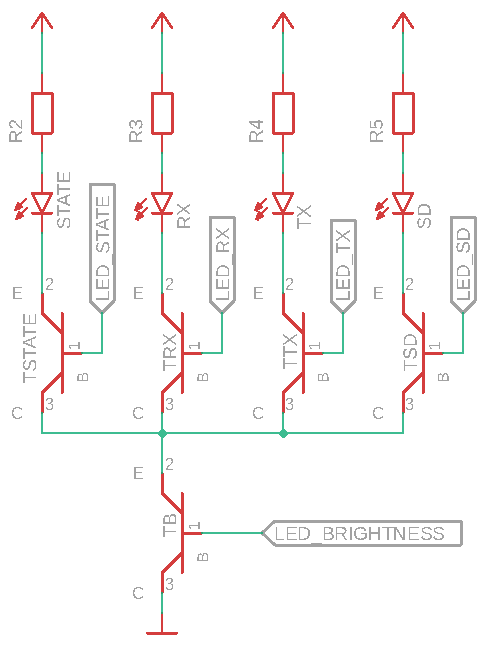
\includegraphics[scale = 0.9]{led-Schaltung}
		\caption{LED Schaltung}
		\label{fig:LED-Schaltung}
	\end{center}
\end{figure}
Abbildung \ref{fig:LED-Schaltung} zeigt die Verschaltung der von dem MCU gesteuerten LEDs. Jede LED wird mit 5\,V Spannung versorgt. Jeweils ein Widerstand begrenzt den Strom, um ein Durchbrennen der LED zu verhindern. Da für die vorhandenen LEDs keine Datenblätter verfügbar sind, werden alle Vorwiderstände mit 120\,Ohm dimensioniert. Das eigentliche Ein- und Ausschalten wird über jeweils einen Transistor realisiert. Die Basen des Transistoren werden mit jeweils einem Ausgang des MCUs verbunden. Der Benutzer soll die Möglichkeit haben, die Helligkeit der LEDs je nach Anforderung zu verändern. Dazu werden die Kollektoren aller LED-Schalttransistoren auf den Emitter eines weiteren Transistors \textit{TB} geschaltet. Die Basis wird mit einem Ausgangspin des MCUs verbunden, der mittels eines Timers ein pulsweitenmoduliertes Signal (PWM-Signal) ausgeben kann. Mithilfe einer Anpassung der Pulsweite kann so die Helligkeit aller LEDs reguliert werden. Je kürzer die Pulsweite ist, also je kürzer die LED eingeschaltet ist, desto weniger hell erscheint sie. Die Frequenz des PWM-Signals muss dabei so hoch sein, dass für das menschliche Auge nicht mehr ersichtlich ist, dass die LED nicht dauerhaft leuchtet.\\
%Hier noch mehr zu PWM schreiben. Verweis aus Kapitel Software/Einstellungen
%Dimensionierung der Vorwiderstände
%In der aktuellen Version des Aufnahmegerätes sind die Vorwiderstände aller LEDs pauschal mit 120\,Ohm dimensioniert, was in stark unterschiedlichen Helligkeiten der einzelnen LEDs resultiert. 
%\begin{figure}[h]
%	\begin{center}	
%		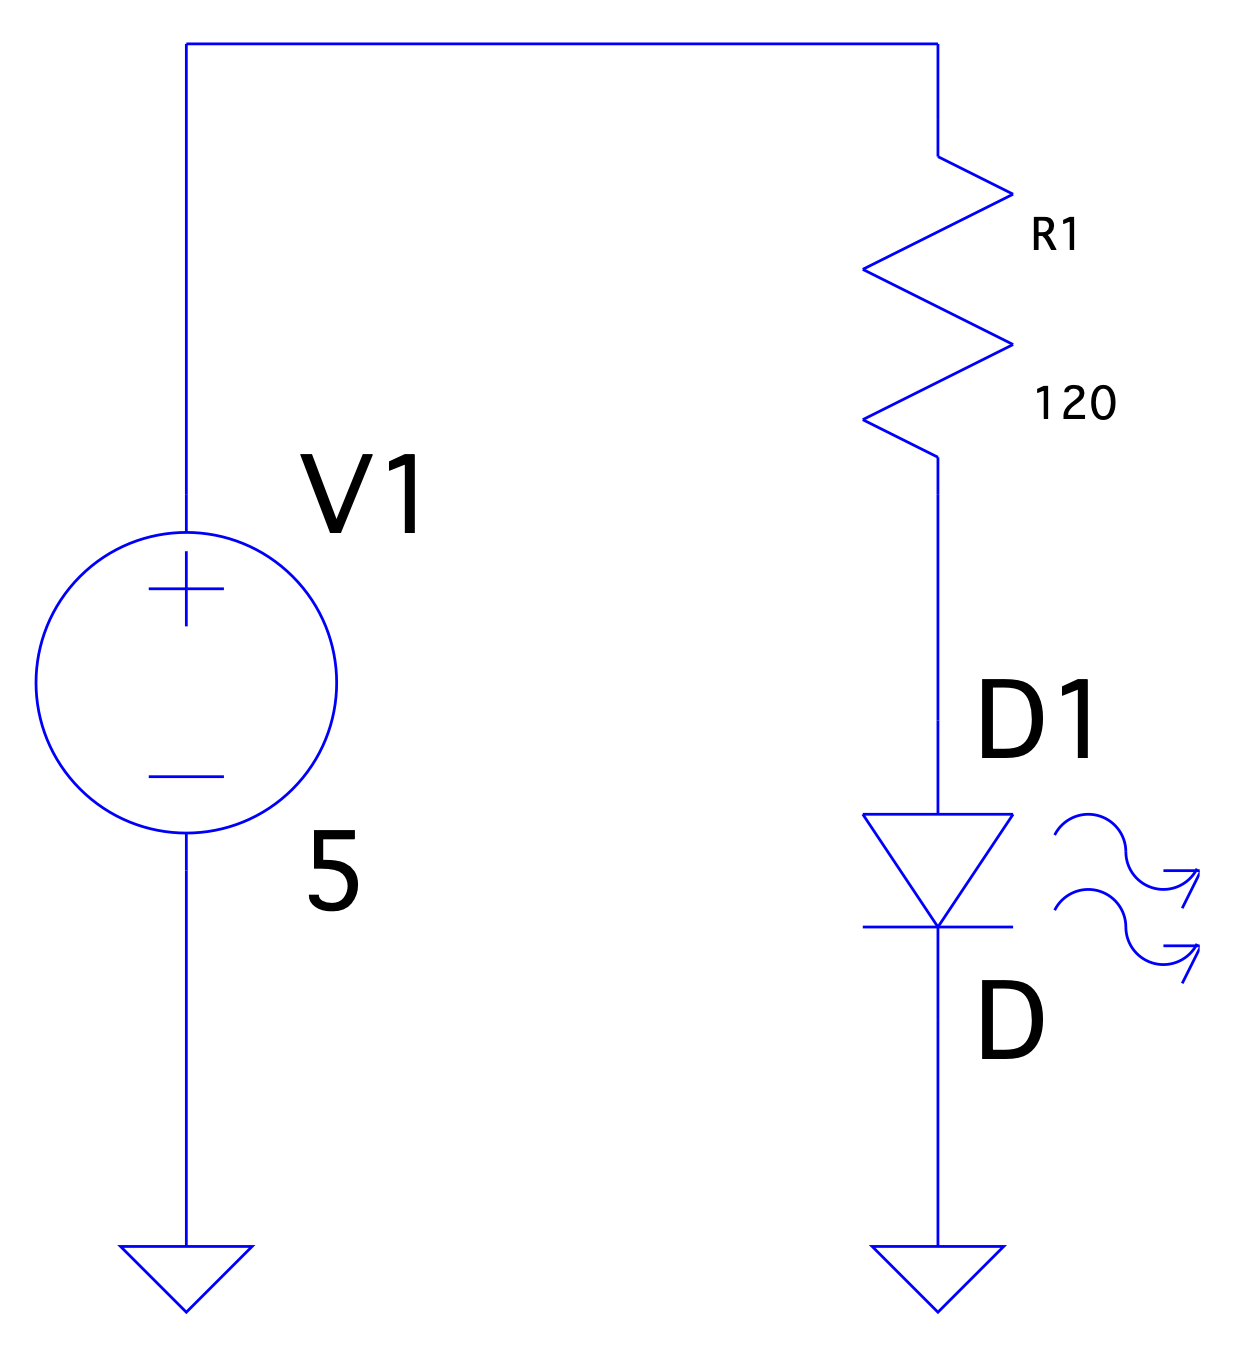
\includegraphics[width=\linewidth/4]{LED-Messung}
%		\caption{LED-Spannungsabfall Messung}
%	\end{center}
%\end{figure}
%
%\begin{table}[h]
%	\begin{center}
%		\begin{tabular}{l | l | l | l}
%			\textbf{LED-Farbe} & \textbf{$U_{LED}$} & $U_R$ & $I_{LED}$\\
%			\hline
%			blau & 3,9\,V & 0,7\,V & 5,83\,mA\\
%			rot & 2,0\,V & 2,6\,V & 21,66\,mA\\
%			grün & 2,5\,V & 1,9\,V & 15,83\,mA\\
%			orange & 2,2\,V & 2,4\,V & 20,00\,mA\\
%		\end{tabular}
%	\caption{Messung mit 120\,Ohm Vorwiderstand}
%	\end{center}
%\end{table}